\documentclass[a4paper]{article}
\usepackage{forest}
\usepackage{float}
\usepackage{geometry}
\usepackage{listings}
\usepackage{hyperref}
\usepackage{graphicx}
\usepackage{ragged2e}
\usepackage{color}
\usepackage{xepersian}
\usepackage{subfiles}
\newgeometry{left=1.4cm, right=1.4cm, bottom=2.0cm, top=2.0cm}
\settextfont[Scale=1]{XB Roya}

\renewcommand{\baselinestretch}{1.5}
\definecolor{dkgreen}{rgb}{0,0.6,0}
\definecolor{gray}{rgb}{0.5,0.5,0.5}
\definecolor{mauve}{rgb}{0.58,0,0.82}
\definecolor{commentColor}{rgb}{0.6,0.6,0.60}

\title{معماری مقیاس بزرگ \\ خانم دکتر سحر آدابی}
\author{علیرضا سلطانی نشان}

\begin{document}
\maketitle
\tableofcontents

\section*{مجوز}

به فایل license همراه این برگه توجه کنید. این برگه تحت مجوز GPLv3 منتشر شده است
که اجازه نشر و استفاده (کد و خروجی/pdf) را رایگان می‌دهد.

\section{پیشگفتار}

اگر درس مهندسی نیازمندی‌ها را خوانده باشید، احتمالاً در جریان آن هستید که برای
تولید نرم‌افزار بخش‌های زیادی درگیر هستند اما در حالت کلی در درس پیشین دانستیم
که در ابتدا بایستی نیازمندی‌های مشتری یا کارفرما را از محصول نرم‌افزار بدانیم،
آن را بررسی و تحلیل کنیم، سند نیازمندی آن را آماده‌سازی کنیم و سپس به دنبال
طراحی معماری آن برویم. در این درس به طراحی و پیاده‌سازی سند معماری مقیاس بزرگ یک
محصول نرم‌افزاری می‌پردازیم تا فرایند تولید نرم‌افزار را به طور کامل طی کرده
باشیم.

\section{معرفی}

\subsection{چه زمانی یک پروژه مقیاس بزرگ است؟}

برای اینکه بتوانیم بگوییم که چه پروژه‌ای مقایس بزرگ محسوب می‌شود، براساس دو
استاندارد ایرانی و بین‌المللی می‌توان دو استاندارد را در اینجا مطرح کرد:

\begin{itemize}
    \item استاندارد مقیاس بزرگ بودن پروژه از نظر دکتر شمس، آن است که پروژه بیشتر
    از ۶ ماه زمان پیا‌ده‌سازی نیاز داشته باشد و تعداد درخواست‌های ارسالی به آن
    ۱۲ نفر به بالا باشد.
    \item استاندارد بین‌المللی مقیاس بزرگ بودن پروژه را زمان یک سال به بالا جهت
    پیاده‌سازی و تعداد درخواست‌ها را بین ۲۰ تا ۲۲ نفر تعیین می‌کند.
\end{itemize}

ابتدایی ترین فاز معماری یک محصول نرم‌افزاری مقیاس بزرگ، طراحی و بررسی و آنالیز
سناریو‌های آن است.

سند معماری نرم‌افزار به مجموعه‌ای از سناریو‌هایی گفته می‌شود که در ازای هر کدام
یک راه‌حل مناسب مطرح می‌شود.

یکی از نیازمندی‌های بررسی معماری نرم‌افزار مقیاس بزرگ استفاده از متدولوژی
\lr{RUP}\footnote{\lr{Rational Unified Process}} می‌باشد. دلیل اصلی آن این است
که می‌توان تمام فرایند‌های آن را به همراه \lr{Artifact}ها شخصی‌سازی کرد. در
معماری نرم‌افزار می‌توانیم مشخص کنیم که چه اجزایی داریم و این اجزا چگونه با
یکدیگر در ارتباط هستند و شامل چه قید‌هایی می‌شود. در حقیقت در سند معماری
نرم‌افزار نمود خارجی المان‌ها را مطرح می‌کنیم. نحوه در کنار هم چیدن سرویس‌ها را
مطرح می‌کنیم اما هیچ وقت در مورد جزئیات اینکه برای مثال از چه الگوریتم‌هایی
استفاده می‌کنیم، صحبت نمی‌شود. در این سند علاوه‌بر نیاز‌های جاری، در مورد
نیاز‌های آتی نیز صحبت می‌شود که در آینده چقدر باید نرم‌افزار قابلیت گسترش
\lr{Expandability} داشته باشد.

\subsection{یادآوری متدولوژوی \lr{RUP}}

این متدولوژوی به عنوان یک متدولوژوی توسعه نرم‌افزار اجایل، به دلیل قابل تکرار
بودنش در نظر گرفته شده است. این روش مهندسی نرم‌افزار از یک سیستم انعطاف پذیر و
سازگار در فرایند توسعه نرم‌افزار استفاده می‌کند که در برگیرنده انجام تنظیمات و
تکرار دوره‌های مهندسی نرم‌افزار است تا زمانی که محصول به نیازمندی‌های مطرح شده و
اهداف برسد \cite{rupStudy}.

\subsubsection{منظور از نظم در \lr{RUP}}

منظور از نظم در حقیقت نمود‌هایی می‌باشد که در فرایند توسعه نرم‌افزار مورد
استفاده قرار می‌گیرد، در حقیقت نظم، مدل‌سازی حرفه‌ای را نشان می‌دهد. این نظم‌ها
به ما کمک می‌کنند که چه زمانی چه \lr{Activity}هایی را باید به چه میزان در چه
بازه‌هایی انجام دهیم و خروجی مورد نظر ما چیست؟

برای مثال در فرایند تحلیل نیازمندی پروژه، نظم نیازمندی، خروجی فاز‌های آن است که
به شکل مدل‌های \lr{Usecase diagram} و سند معماری نرم‌افزار کشیده و نوشته شده
است.

\subsubsection{چهار فاز اصلی در \lr{RUP}}

\begin{enumerate}
    \item فاز آغاز یا \lr{Inception}: در این فاز تمام نیازمندی‌ها جمع‌آوری
    می‌شود و مقیاس پروژه در آن بدست می‌آید.
    \item فاز توسعه یا \lr{Elaboration}: طراحی سیستم و تحلیل دقیق‌تر نیازمندی‌ها
    صورت می‌گیرد.
    \begin{enumerate}
        \item استفاده از مدل‌سازی‌ها و کشیدن دیاگرام‌ها
        \item کشیدن مدل \lr{usecase}: کاربرد بزرگی برای مشتری (کارفرما) و طراح
        دارد و برای هر دو طرف قابل فهم می‌باشد. در این نوع نمودار افعال و
        نیازمندی‌های \lr{functional} مطرح می‌شود. انتظارات در مورد سیستم در
        اینجا مورد بحث قرار می‌گیرند.
        \begin{itemize}
            \item اینکه کاربرد بتواند زیر ۲ ثانیه احراز هویت شود مربوط به
            نیازمندی‌های \lr{non-functional} می‌باشد.
            \item شامل دو سند می‌شود:
            \begin{itemize}
                \item سند \lr{Usecase} که انتظارات سیستم را مشخص می‌کند.
                \item سند معماری که \lr{function} و \lr{non-functional} را در بر
                می‌گیرد.
            \end{itemize}
        \end{itemize}
        \item طراحی \lr{Class diagram} 
        \item طراحی \lr{Sequence diagram}
    \end{enumerate}
    \item فاز ساخت یا \lr{Construction}: در این فاز کد نویسی و ارزیابی کد‌های
    نوشته شده صورت می‌گیرد.
    \item فاز استقرار یا \lr{Deployment}: در این فاز نرم‌افزار آماده شده است و
    در بستری مناسب به کاربران نهایی \footnote{\lr{End users}} ارائه می‌شود که
    نیازمند آموزش‌های لازم می‌باشد.
\end{enumerate}

محبوبیت استفاده از متدولوژی \lr{RUP} به خاطر آن است که کاملاً به صورت جامع سیستم
را در بر می‌گیرد.

\subsubsection{منظور از فرسخ‌شمار چیست؟}

فرسخ‌شمار یا \lr{Milestone} در هر کدام از فاز‌ها مشخص می‌شود که در حقیقت در مورد
تعیین یک بازه زمانی مشخص صحبت می‌کند. در آن می‌توانیم ببینیم که در فاز‌های قبلی
چه کار‌هایی بایستی انجام می‌شده، آیا آن‌ها را انجام داده‌ایم و اگر انجام
نداده‌ایم یا مشکلی در آن وجود دارد آن فاز را تکرار می‌کنیم تا به انتهای آن برسیم
که به نحوی تسک یا وظیفه را ببندیم.

\subsubsection*{نکات}

\begin{itemize}
    \item ساده‌ترین سند در میان این ۴ فاز، سند استقرار می‌باشد.
    \item معماری مقیاس‌پذیر (بزرگ) یک پروژه نرم‌افزار دو بُعد پویا و ثابت دارد.
    \item در مورد ارزیابی کارایی و آزمون نرم‌افزار گفتنی است که هر توسعه‌دهنده
    مسئول \lr{Quality control} بخش خودش است.
    \item تکرار‌ها \lr{n} تا هستند مدیر پروژه یا طراح سیستم باید به ما تعداد
    تکرار‌ها را به صورت تقریبی بگوید.
\end{itemize}

\subsubsection{محوریت بر روی نیازمندی‌ها}

متدولوژوی \lr{RUP} تاکید زیادی روی شناسایی و مدیریت نیازمندی‌ها را دارد و به
تیم‌ها کمک می‌‌کند تا نیازمندی‌های کلیدی پروژه‌ را به خوبی درک و پیاده‌سازی
کنند.

\subsubsection{استفاده از برنامه‌نویسی \lr{OOP}}

این متدولوژی به طور گسترده از ۴ اصل شیء‌گرایی استفاده می‌کند و به توسعه‌دهندگان
اجازه می‌دهد که کد‌های قابل استفاده مجدد و مدیریت فاکتور‌های انعطاف پذیری را
ایجاد کنند.

\section{معماری مقیاس بزرگ نرم‌افزار}

\subsection{معماری نرم‌افزار چیست؟}

معماری نرم‌افزار یک تعریف واحد ندارد. معماری نرم‌افزار یک برنامه یا یک سیستم
محاسباتی می‌باشد. یک ساختار یا مجموعه ساختار‌هایی است از سیستم مورد نظر ما که
متشکل از المان‌های کامپیوتری است و نمود خارجی یک چیز (المان) می‌باشد و ارتباطات
بین آن‌ها را در بر می‌گیرد. هیچ‌گاه نمی‌توان نرم‌افزاری نوشت که معماری نرم‌افزار
نداشته باشد. برای مثال از معماری \lr{MVC} در نرم‌افزار خود استفاده کرده‌ایم.
نرم‌افزاری وجود ندارد که معماری نداشته باشد. اگر بگوییم نرم‌افزاری معماری ندارد
در حقیقت علم معماری به کار گرفته شده را نمی‌دانیم که آن را بی‌معماری می‌نامیم.
برای مثال معماری کلاینت سرور که براساس نیازمندی‌های نرم‌افزاری بیان می‌شود که چه
بخش‌هایی سمت سرور باشد چه‌ بخش‌هایی سمت کلاینت.

\subsection{معمار نرم‌افزار کیست؟}

معمار نرم‌افزار شخصی مدبر است که تجربه تخصصی آن در حوزه‌ای مشخص بیشتر از ۱۰ سال
است که تسلط کافی در آن سیستم مشخص دارد و از ابتدا تا انتهای پروژه با فرایند
توسعه و توسعه‌دهندگان همراه است.

\subsection{المان‌ها}

بخش‌های یک سیستم نرم‌افزاری را گویند برای مثال یک نرم‌افزار واحد مانیتورینگ،
واحد زمان‌بندی، واحد بررسی درخواست‌ها و غیره را دارد.

\subsection{\lr{External Feasible Properties}}

آن بخش چه وظیفه‌ای را باید انجام دهد و آن بخش آن وظیفه را در حال انجام است یا
خیر؟ جزئیات مربوط به المان‌های درگیر در بخش معماری در \lr{External Feasible
Properties} مطرح نمی‌شود.

\subsection{تفاوت کامپوننت و المان}

وقتی در مورد کامپوننت می‌گوییم در حقیقت چیزی است که می‌خواهیم آن را پیاده‌سازی
کنیم. المان کامپوننتی است که قسمت اجرایی را برای آن در نظر نگرفته‌ایم.

\subsection{بخش‌هایی که معماری نرم‌افزار باید پوشش دهد}

\begin{enumerate}
    \item المان‌هایی که در سیستم قرار است استفاده شود را مشخص می‌کند.
    \item نمود خارجی المان‌های سیستم مورد نظر را مشخص می‌کند و تعیین می‌کند هر
    المانی در سیستم چه وظیفه‌ای را انجام دهد.
    \item ارتباطات بین المان‌ها را به روشنی مشخص می‌کند.
\end{enumerate}

در کنار تمامی موارد بالا، بخش‌هایی که یک معماری نرم‌افزار پوشش نمی‌دهد شامل ذات
المان‌ها می‌باشد.

\subsection{قابلیت اطمینان یا \lr{Reliability}}

یک سیستمی که در زمان مشخص درست کار کند به شرطی که در زمان $T - x$ درست کار کرده
باشد.

\subsection{قابلیت استفاده یا \lr{Useability}}

سیستمی که کارآمد باشد برای آن دسته از افرادی که سیستم را حاضر و آماده کرده‌ایم.
به گونه‌ای که با ظاهر مناسب کار کردن با آن نیز آسان باشد.

\subsection{ارائه سریع محصول یا \lr{Short time to market}}

قابلیت یا \lr{Feature} مجموعه‌ای از توابع نرم‌افزاری است که وقتی در بازار ارائه
می‌شود، واقعاً کار می‌کند. 

\subsubsection*{نکات}

\begin{itemize}
    \item تا آنجایی که می‌شود هزینه‌ها را باید کاهش بدهیم و بیشترین هزینه‌ها را
    ما در بخش توسعه نرم‌افزار خواهیم داشت. همیشه باید کارمندان را مشغول توسعه
    نگهداریم تا باعث از دست رفتن هزینه‌ها نشود.
    \item مشکل معمار آن است که حجم زیادی از نیازمندی‌های نرم‌افزاری را در حال
    بررسی است که نسبت به هم در تضاد هستند.
    \item بخشی از وظایف اصلی معماری نرم‌افزار مشخص کردن استک‌های نرم‌افزاری
    می‌باشد. بخش دیگری از آن این است که بررسی کند این موارد توسط تیم اجرا و
    استفاده می‌شود یا خیر (\lr{Follow up})
\end{itemize}

\subsection{تفاوت معماری سازمانی و معماری نرم‌افزار}

معماری سازمانی و معماری نرم‌افزار با یکدیگر متفاوت است. در معماری سازمانی، چارت
سازمانی آن مشخص‌کننده محدوده و کلیت هر قسمت آن سازمان می‌باشد.

% \lr{Mobile Adhoc Network}

% شبکه‌های موردی متحرک

% یک شبکه‌ای است فاقد زیرساخت. بیشتر در مناطق جنگی و \lr{Real-time} مورد استفاده
% قرار می‌گیرد که بتوانیم در حال حاضر یک شبکه را آماده کنیم که سربازان با یکدیگر
% ارتباط بگیرند به گونه‌ای که \lr{Mobility} بیان می‌کند که شبکه را بایستی با
% زیرساخت مناسب ایجاد کند.

% یک پیام «سلام» ارسال می‌کند و منتظر دریافت \lr{ACK} می‌باشد و بعد از آن سعی
% می‌کند که ارتباط را حفظ کند تا آن کانال ارتباطی بین سربازان برقرار باشد.

\subsection{جزئیات فعالیت‌های معماری نرم‌افزار}

\subsubsection{ساخت \lr{Business case} برای سیستم}

\subsubsection*{یادآوری \lr{Business plan}}
بیزینس پلن سندی است که چهارچوب سیستم ما را در بر می‌گیرد و آن را نسبت به سیستم
مشابه مقایسه می‌کند و آن را به چالش می‌کشد. نسبت به هر چالشی که در سیستم ما وجود
دارد بایستی پاسخی مطرح شده باشد.

سند \lr{Business case} سندی از جنس مالی است که در آن برآورد هزینه و توجیهات
اقتصادی بیان شده است. در این سند، درگیر بودن نیرو‌ها بررسی می‌شود و در نهایت
توجیهات‌ اقتصادی را از نظر کاهش هزینه‌ها مطرح می‌کند. برای مثال ممکن است بیشتر
اوقات بهره‌وری سیستم را افزایش داده باشیم که نسبت به این افزایش باید توجیهی وجود
داشته باشد.

از ابتدا تا انتهای پروژه دائماً در حال تخمین قیمت پروژه به عنوان معمار نرم‌افزار
هستیم که در آن هزینه‌ای را مطرح می‌کنیم که بررسی کرده‌ایم در توسعه نرم‌افزار
نیاز خواهد شد. در این حین اگر هزینه توسعه بیشتر شود باعث ضرر ما و اگر کمتر شود
باعث سود ما خواهد شد. پس به همین دلیل سعی می‌کنیم سند \lr{Business case} را از
ابتدا تا انتهای فرایند پروژه توسعه دهیم و توجیه اقتصادی به روزی در آن داشته
باشیم که موجب ضرر از سمت پیمانکار نشود.

\subsubsection*{نقطه سر به سر یا \lr{Break event point}}

وضعیتی است که در آن هزینه‌هایی که ما برآورد کرده‌ایم در بازه زمانی مشخص، برابر
با صفر شده است. برای مثال اگر مبلغ ۵۰۰ میلیون تومان را به عنوان هزینه نرم‌افزار
محاسبه کرده باشیم و طی یک سال دیگر سازمان دقیقاً همان مبلغ را بدون کاهش یا
افزایش پرداخت می‌کند این وضعیت نقطه سر به سر خواهد شد. زمان نقطه سر به سر
معمولاً در بازه ۲ تا ۵ سال تعریف می‌شود که در واقعیت زمان خیلی طولانی برای تخمین
هزینه توسعه نرم‌افزار محسوب می‌شود.

\subsubsection{فهمیدن نیازمندی‌های پروژه}

نیازمندی‌ها تنها متغیر ثابت هستند. همانطور که پیش‌تر اشاره شد
\lr{non-functional}ها در قالب سند معماری نرم‌افزار دیده می‌شوند. همچنین اگر
نیازمندی \lr{functional} وجود نداشته باشد \lr{non-function}ها معنایی ندارند.
برای مثال می‌گوییم که نرم‌افزارمان بایستی امن باشد، یعنی \lr{Usecase diagram}
داریم که ازای آن نیازمندی \lr{non-function} تعریف کرده‌ایم.

نکته مهم آن است که مهمار نرم‌افزار تنها نیازمندی‌های جاری را در نظر نمی‌گیرد
بلکه نیازمندی‌های آتی را هم در سند پیشبینی می‌کند تا بتواند یک جریان را کامل کند
و به نوعی \lr{Proof of concept} داشته باشد.

\subsubsection{ایجاد یا انتخاب یک معماری نرم‌افزار}

معمار نرم‌افزار معمولاً یا یک معماری را انتخاب می‌کند یا آن را از نو می‌سازد.
ممکن است در تز‌های آکادمیک معماری جدیدی را ایجاد کرده باشیم زیرا ممکن است صورت
مسئله‌های جدیدی پدید آمده باشند یا نیازمندی‌های \lr{non-function} جدیدی یافت شده
باشد. در حالت کلی معماری‌ها را یا باید بهینه‌سازی کنیم یا اجرا و در پروژه
نرم‌افزاری پیاده کنیم.

\subsubsection{دنبال کردن معماری یا \lr{Communicating the architecture}}

چیزی که در معماری نرم‌افزار بیان شده است را دنبال کنیم و بررسی کنیم که تمام آن
فرایند‌های مهندسی توسعه نرم‌افزار را توسعه‌دهنده‌ای دنبال می‌کند یا خیر. بیان
این مسئله طرف معمار و اجرای آن در طرفی دیگر است. خیلی با بخش \lr{Implementing
based on the architecture} ارتباط دارد.

\subsubsection{بررسی و ارزیابی معماری}

نکته مهم آن است که در حوزه معماری نرم‌افزار چیزی به نام شبیه‌سازی نداریم چرا که
قدم ابتدایی هر پروژه‌ای تعیین معماری آن است. اینکه از ما سوال شود که معماری
نرم‌افزارتان را با چه شبیه‌سازی اجرا کردین یا با چه فاکتور‌های شبیه‌سازی آن را
ارزیابی کرده‌اید، بحث کاملاً غلطی می‌باشد. مقایسه بین الگوریتم‌ها امکان‌پذیر
می‌باشد زیرا داریم شبیه‌سازی ورکلود‌ها را انجام می‌دهیم.

در این خصوص روشی را داریم به نام \lr{ATAM} که ارزیابی معماری نرم‌افزار را
می‌توان از طریق آن انجام داد. یک استاندارد مشابه با \lr{ISO} می‌ماند که
نیازمندی‌های \lr{non-functional} را در نظر می‌گیرد. یک تیم مستقل با آن همراه است
که بررسی کند ما از راه درستی استفاده کرده‌ایم یا خیر. در نهایت به ما نشان می‌دهد
که نسبت به آن سناریو می‌توانیم این معماری را پوشش دهیم یا خیر.

برای بررسی و ارزیابی معماری راه‌های مختلفی وجود دارد:

\begin{enumerate}
    \item مدل‌سازی صوری، فرمال و رسمی: برای اینکه ثابت کنیم چیزی که داریم
    می‌نویسم قابل تایید است و درست می‌باشد. به دلیل آن که ریاضی هستند می‌توانند
    مفید و رویکردی مناسب باشند.
    \item استفاده از \lr{ADL: Architecture Definition Language}
    \item استفاده از \lr{Prototype}ها: اگر یک سیستم کوچک درست کنیم که به
    صورت صحیح کار کند می‌تواند نشان دهنده آن باشد که سیستم اگر بزرگتر شود هم
    صحیح کار خواهد کرد.
    \item ۸۰ درصد نیازمندی‌ها و دامنه‌های مسئله با نرم‌افزاری که در حال کار است
    که با این معماری انطباق دارد پس قطعاً معماری با کار‌های آینده ما نیز منطبق
    خواهد بود.
\end{enumerate}

\subsubsection*{نکته}

دامنه مسئله مثل دامنه سیستم‌های مالی، دامنه سیستم‌های آموزشی و غیره یک تعریف
مسئله مخصوص و واحد دارد که در سیستم‌های گوناگون مشابه یکدیگر هستند و دقیقاً
نیازمندی‌های آن‌ها نیز مشابه هستند. اگر یک سیستم مشابه را پیدا کردیم، معماری
انتخابی ما می‌تواند با سیستم مشابه نیز کار کند.

\subsubsection{پیاده‌سازی مبتنی بر معماری}

بررسی اینکه آیا تمام فرایند‌هایی که در فاز‌های توسعه نرم‌افزار شروع می‌شود با
بیانات و نقشه‌راه معمار نرم‌افزار مطابقت دارد یا خیر؟

\subsubsection{اطمینان از انطباق نسبت به یک معماری}

در این بخش بررسی می‌کنیم که فرایند‌ها تماماً تابعی از معماری هستند یا خیر؟ در
انتهای کار، تمام‌ اسناد را در کنار هم قرار می‌دهیم و به تطبیق اسناد با سند
معماری می‌پردازیم. برای مثال تمام \lr{Usecase diagram}ها مطابق با سند معمعاری
\lr{Usecase}ها بوده‌اند؟ طبق استاندارد طراحی شده‌اند؟ اگر هر کدام مطابقت نداشت
بایستی سریعاً اصلاح شود تا از ایجاد هزینه‌های آینده جلوگیری به عمل آورد. ما
بایستی مطمئن باشیم که تمام اسنادی که به معمار نرم‌افزار تحویل می‌دهیم مطابق با
سند معماری باشد که شامل چندین بخش خواهد شد.

\subsection{چه چیزی یک معماری خوب را تحویل می‌دهد؟}

هیچ چیز ذاتاً خوب یا بد نیست بلکه واسبتگی بسیار زیادی به کاربرد آن در سیستم مورد
نظر دارد. معماری کنترل دمای یک نیروگاه تولید برق را نمی‌توان در کنترل دمای خانه
استفاده کرد چون استفاده نادرست و نا به جایی بوده است. ذاتاً نمی‌توانیم بگوییم که
کدام معماری خوب است کدام معماری بد بلکه انتخاب ما نسبت به سیستم خوب و بد دارد.

معماری قابل ارزیابی است پس باید براساس اهدافی که داریم فرایند ارزیابی را انجام
دهیم تا در نهایت ببینیم که این ارزیابی چقدر می‌تواند معماری را با اهداف ما
\lr{Match} کند. برای مثال ممکن نیست که یک سامانه‌ای که امنیت ندارد را الهام
بگیریم برای سامانه‌ای که یکی از اهداف اصلی آن امنیت است.

نمودار زیر را از معماری سطح بالای \lr{ATM} را در نظر بگیرید:

\begin{figure}[H]
    \centering
    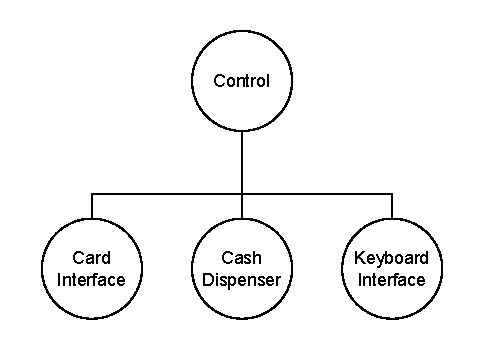
\includegraphics[width=0.5\textwidth]{images/bad-arch-of-atm.drawio.pdf}
    \caption{نمایش معماری سطح بالا دستگاه \lr{ATM}}
    \label{fig:atmDiagram}
\end{figure}

شکل شماره \ref{fig:atmDiagram} ساختار کلی از دستگاه \lr{ATM} را نمایش می‌دهد.
درست است که در مطالب بالاتر گفتیم که معماری یک چکیده از ساختار سیستم می‌باشد اما
در این نمودار ارتباطات بین المان‌ها کاملاً همراه با ابهام می‌باشد و تمام معماری
دستگاه \lr{ATM} را پوشش نمی‌دهد. در این نمودار ذات المان‌ها مشخص نیست. برای مثال
مشخص نیست که واحد \lr{Card interface} ممکن است هم کارت را دریافت کند هم اعتبار
کارت ورودی را بسنجد؟ پس می‌توان گفت وظیفه المان \lr{Card interface} در این
نمودار اصلاً مشخص نیست و در این نمودار دقیقاً ماهیت ارتباطات بین المان‌ها مشخص
نیست. همچنین لایه‌بندی در این نمودار به صورت واضح کشیده نشده است. در لایه‌بندی
همواره منطق وجود دارد مانند لایه‌بندی استاندارد \lr{OSI} که جانمایی المان‌ها در
این نمودار کامل کشیده نشده است. برای مثال بحث امنیت و کارایی و تعامل‌پذیری اصلاً
وجود ندارد. لایه‌بندی یک معماری تماماً توسط معمار نرم‌افزار مشخص خواهد شد.

\subsection{تفاوت \lr{Fault} با \lr{Failure}}

\lr{Fault} یعنی یک نقضی بالقوه در سیستم وجود دارد تا زمانی که سیستم بدون مشکل
کار کند آن نقض خودش را نمایان نمی‌کند اما در شرایط خاصی ممکن است برنامه به این
\lr{Falut} برخورد کند و بالفعل موجب از کار افتادن نرم‌افزار شود. در حقیقت بعد از
برخورد نرم‌افزار با \lr{Fault} پدیده‌ای به نام \lr{Failure} رخ می‌دهد. در حقیقت
\lr{Fault} در نرم‌افزار وجود داشته است که در شرایط خاص با ورودی خاص کاربر برنامه
با شکست یا \lr{Failure} رو به رو می‌شود و باعث کار نکردن درست نرم‌افزار خواهد
شد.

همواره \lr{Fault} از سمت طراحی نرم‌افزار همراه خواهد بود زیرا بایستی در اسناد
طراحی به آن نگاه مهندسی شود. زمانی که پیاده‌سازی می‌شود اگر در شرایط آزمون
بتوانیم آن \lr{Fault}ها را شناسایی کنیم و آن‌ها را رفع کنیم سیستم را از
\lr{Failure}های آینده نجات خواهیم داد.

نکته: \lr{Fault} موجب \lr{Failure} می‌شود.

اگر ما یک حافظه \lr{USB} داشته باشیم و در هنگام انتقال اطلاعات ناگهانی فلش را از
سیستم خارج کنیم، در حقیقت نه \lr{Fault} نه \lr{Failure} و نه \lr{Error} رخ داده
است. بلکه سیستم توسط عامل خارجی دستکاری شده است. اگر \lr{Fault} در سیستم داشته
باشیم بایستی توانایی هندل کردن آن را در نرم‌افزار داشته باشیم.

\subsection*{نکات}

\begin{itemize}
    \item معماری نرم‌افزار المان‌های نرم‌افزاری را مشخص می‌کند.
    \item \lr{Mapping} تسک‌ها به منبع مشخص تعریف زمانبندی است.
    \item تسک‌ها در حقیقت کار‌هایی هستند که در سیستم تعریف می‌شوند.
    \item ورکفلو مجموعه‌ای از تسک‌های وابسته به هم می‌باشد.
    \item \lr{Bag of tasks} عموماً وابستگی ندارند.
    \item \lr{Multiple workflow scheduling} به معنای زمانبندی چند ورکفلو
    می‌باشد.
    \item همیشه یک زمانبندی بهینه نداریم بلکه باید در شرایط مناسب از زمانبندی
    مناسبی استفاده کنیم.
    \item در هنگام مهندسی نرم‌افزار باید تا آنجایی که می‌شود نرخ موفقیت یک تسک
    را بالا ببریم.
\end{itemize}

\subsection{منابع همگن و ناهمگن}

\begin{itemize}
    \item منابع همگن به منابعی گفته می‌شود که همه المان‌ها در آن دقیقاً یک چیز
    هستند یا به عبارتی همه منابع به صورت \lr{Clone} از یکدیگر هستند. برای مثال
    همه از یک سخت‌افزار استفاده می‌کنیم بدون هیچ تفاوتی.
    \item منابع ناهمگن به متفاوت بودن سیستم‌ها نسبت به یکدیگر اشاره دارد.
\end{itemize}

\newpage
\bibliographystyle{unsrt-fa}
\bibliography{refs.bib}
\end{document}